%!TEX encoding = UTF-8 Unicode
%!TEX program = xelatex

\documentclass[bachelor]{ustcthesis}
% bachelor|master|doctor
\usepackage{ustcextra}
\graphicspath{{figures/}}
\bibliographystyle{ustcauthoryear}
% \bibliographystyle{ustcnumerical}


\newcommand{\docname}{即时通讯系统}
\renewpagestyle{front}[\zihao{-5}]{
    \sethead{}{\docname 需求规格说明书}{}
    \setfoot{}{\thepage}{}
    \headrule
}
\renewpagestyle{main}[\zihao{-5}]{
    \sethead{}{\docname 需求规格说明书}{}
    \setfoot{}{\thepage}{}
    \headrule
}
\newcommand{\HRule}{\rule{\linewidth}{0.5mm}}

\begin{document}



\begin{titlepage}
\begin{center}
~\\[5cm]
\HRule \\[0.4cm]
{\huge \bfseries \docname\\需求规格说明书}\\[0.4cm]
\HRule \\[1.5cm]

\begin{tabular}{ccc}
  & 人员 & 日期 \\ 
 &  戴路  &  \\ 
拟制 &  张劲暾 & 2019-04-18 \\ 
 &  王浩宇 &  \\ 
%评审人 & • & yyyy-mm-dd \\ 
%批准 & • & yyyy-mm-dd \\ 
%签发 & • & yyyy-mm-dd \\ 
\end{tabular} 

\end{center}
\end{titlepage}



\frontmatter
\begin{abstract}
%================== 摘要 ===============================
本文档是一份即时通讯系统的设计概要,包括即时通讯系
统的任务概述、总体设计、接口设计、数据结构设计、数据库设计、界面设计、
出错处理设计和维护设计等详细描述。本文档可以为项目开发和维护人员提供参考手册。本文档的预期读者为系统设计人员、软件开发人员、客户方的系统设计人员和项目评审人员。


\textbf{关键词:} 即时通讯系统\quad 团队工作\quad 设计\quad 开发\quad Java\quad 网络通信 \quad
%=======================================================
\begin{table}[htbp]
\centering
\caption{缩略词清单} \label{tab:simpletable}
\begin{tabular}{|c|c|c|}
    \hline
    缩略语 & 英文全名 & 中文解释 \\
    \hline
    CPU & Central Processing Unit & 中央处理器\\
    \hline
    API & Application Programming Interface & 应用程序编程接口\\
    \hline
    DB & Database & 数据库 \\
    \hline
\end{tabular}
\end{table}
%=======================================================
\end{abstract}

\tableofcontents
\listoffigures
\listoftables
% \listofalgorithms  % 算法索引,如不需要,可直接注释掉本行
% \begin{notation}

%\centering
%XX 软件需求规格说明书

%关键词:能够体现文档描述内容主要方面的词汇。
 
%摘要:


\centering
\begin{tabular}{rl}
$\ln x$ & natural logarithm $\log_ex$ \\
$\log x$ & common logarithm $\log_{10}x$ \\
$x\ \mathrm{mod}\ y$ & remainder \\
\end{tabular}

\end{notation}


\mainmatter
\chapter{简介}
\section{目的}
% This section should state the purpose of the document. It could also specify the intended audience. Identify the product whose software requirements are specified in this document.

% 这部分要描述文档的目的。应该指明读者。说明本需求文档描述了哪个产品的软件需求。

现代工作团队,包括高校学生团体,课堂组织,班级管理,科研团队,企业部门,开发团队,工作小组等对于即时通讯系统
有着专业的、高质量的应用需求。能够提供高效、专业、功能强大、扩展性好的即时通讯系统对于提高
工作团队工作效率和管理水平有着重要意义。本产品将降低信息管理和通讯代价,为不同情境下的即时通讯需求
提供解决方案,包括对于一对一即时通讯(私聊)功能、情境群聊功能、个人日程管理、活动/任务发布,音视频通话/会议、
广播/公告板功能,个性化好友推荐,在线文档写作平台等工作团队需求度较高的需求的解决方案。

\section{范围}
% This section should address areas which this document includes and that are specifically excludes. 

% 本节应描述文档所包括和不包括的内容。
    本文档包括对于用户需求的分析和产品功能的介绍,描述各项功能的具体需求,约束和限制,流程,依赖关系,
    为即时通讯系统的设计、实现、测试以及验收提供重要依据,也为评价系统功能和性能
    提供标准。本文档可供用户、项目管理人员、系统分析人员、程序设计人员以及
    系统测试人员阅读和参考。

\chapter{总体概述}
%======================================================================================
% 本节描述影响产品和产品需求的一般因素。由以下4个部分构成。 
% 有一点需说明的是本节不描述具体的需求,只是使那些将要描述的具体需求更易于理解。
%======================================================================================
\section{软件概述}

	\subsection{项目介绍}
	%======================================================================================
	% 描述本软件需求所描述的项目的背景。
	% 例如:本项目是一系列版本中的一个,或者是替代某个已经存在的系统,还是一个新的独立的项目。
	%======================================================================================
	本项目是一个新的独立的项目,旨在为现代高校和企业工作团队提供一个完整高效的即时通讯系统平台;
	实现通讯,管理,公告,文件的在线支持;
	使得工作团队可以随时随地交流信息,协同合作;
	方便团队的组织和事务、活动信息的发布;
	为个人资料管理和日程安排提供高效工具。

	\subsection{产品环境介绍}
	%=========================================gongnneg=============================================
	% 描述的是本产品与其它产品或项目所组成的整体环境。
	% 1.如果本产品是独立的并完全自我包含,在此说明这一点。
	% 2.如果SRS定义的产品是更大的系统或项目的组件(此种情形经常发生),那么应:
	%	A. 	描述此大系统或项目每个组件的功能,并且标识接口。
	%	B. 	确定本软件产品主要外部接口。
	%		(注意:在此部分并不进行这些接口的详细描述;对这些接口的详细描述在SRS的其它部分提供。)
    %	C. 	描述相关产品硬件和所使用的外部设备。(注意:这只是概述性描述。)
	% 通过方块图来描述大系统或项目的主要组件,互连性以及外部接口将是非常有帮助的。
	% 本部分不应提出一个具体的设计解决方案或对解决方案的具体设计约束(具体设计约束将在具体需求章节中描述)。
	% 本部分内容是产生设计约束的基础。
	%======================================================================================
	本产品是一个相对独立的的产品,可以独立运行实现绝大多数核心功能需求,
	扩展性功能进一步支持邮箱管理,需要的其他组件是邮箱组件,包括登录认证,接收邮件和发送邮件
	功能接口,不需要其他外部设备。
\newpage
\section{软件功能}
%======================================================================================
% 概述软件的必须实现的和通过用户操作实现的主要功能。
% 这里只需要进行简要描述(例如目录列表),详细描述在详细需求部分描述。
% 对需求功能进行组织,以便于读者理解,并能指导后续的设计和测试。
% 可以用图表来表示主要需求群组之间的关系,例如:高层的数据流图,面向对象的分析等。
% 有时此部分所要求的功能概述可以从分配具体功能给此软件产品的更高层规格(如果存在的话)直接引用。
% 本节不应描述具体需求。但本节内容是具体需求章节的基础。
%======================================================================================
\begin{center}
	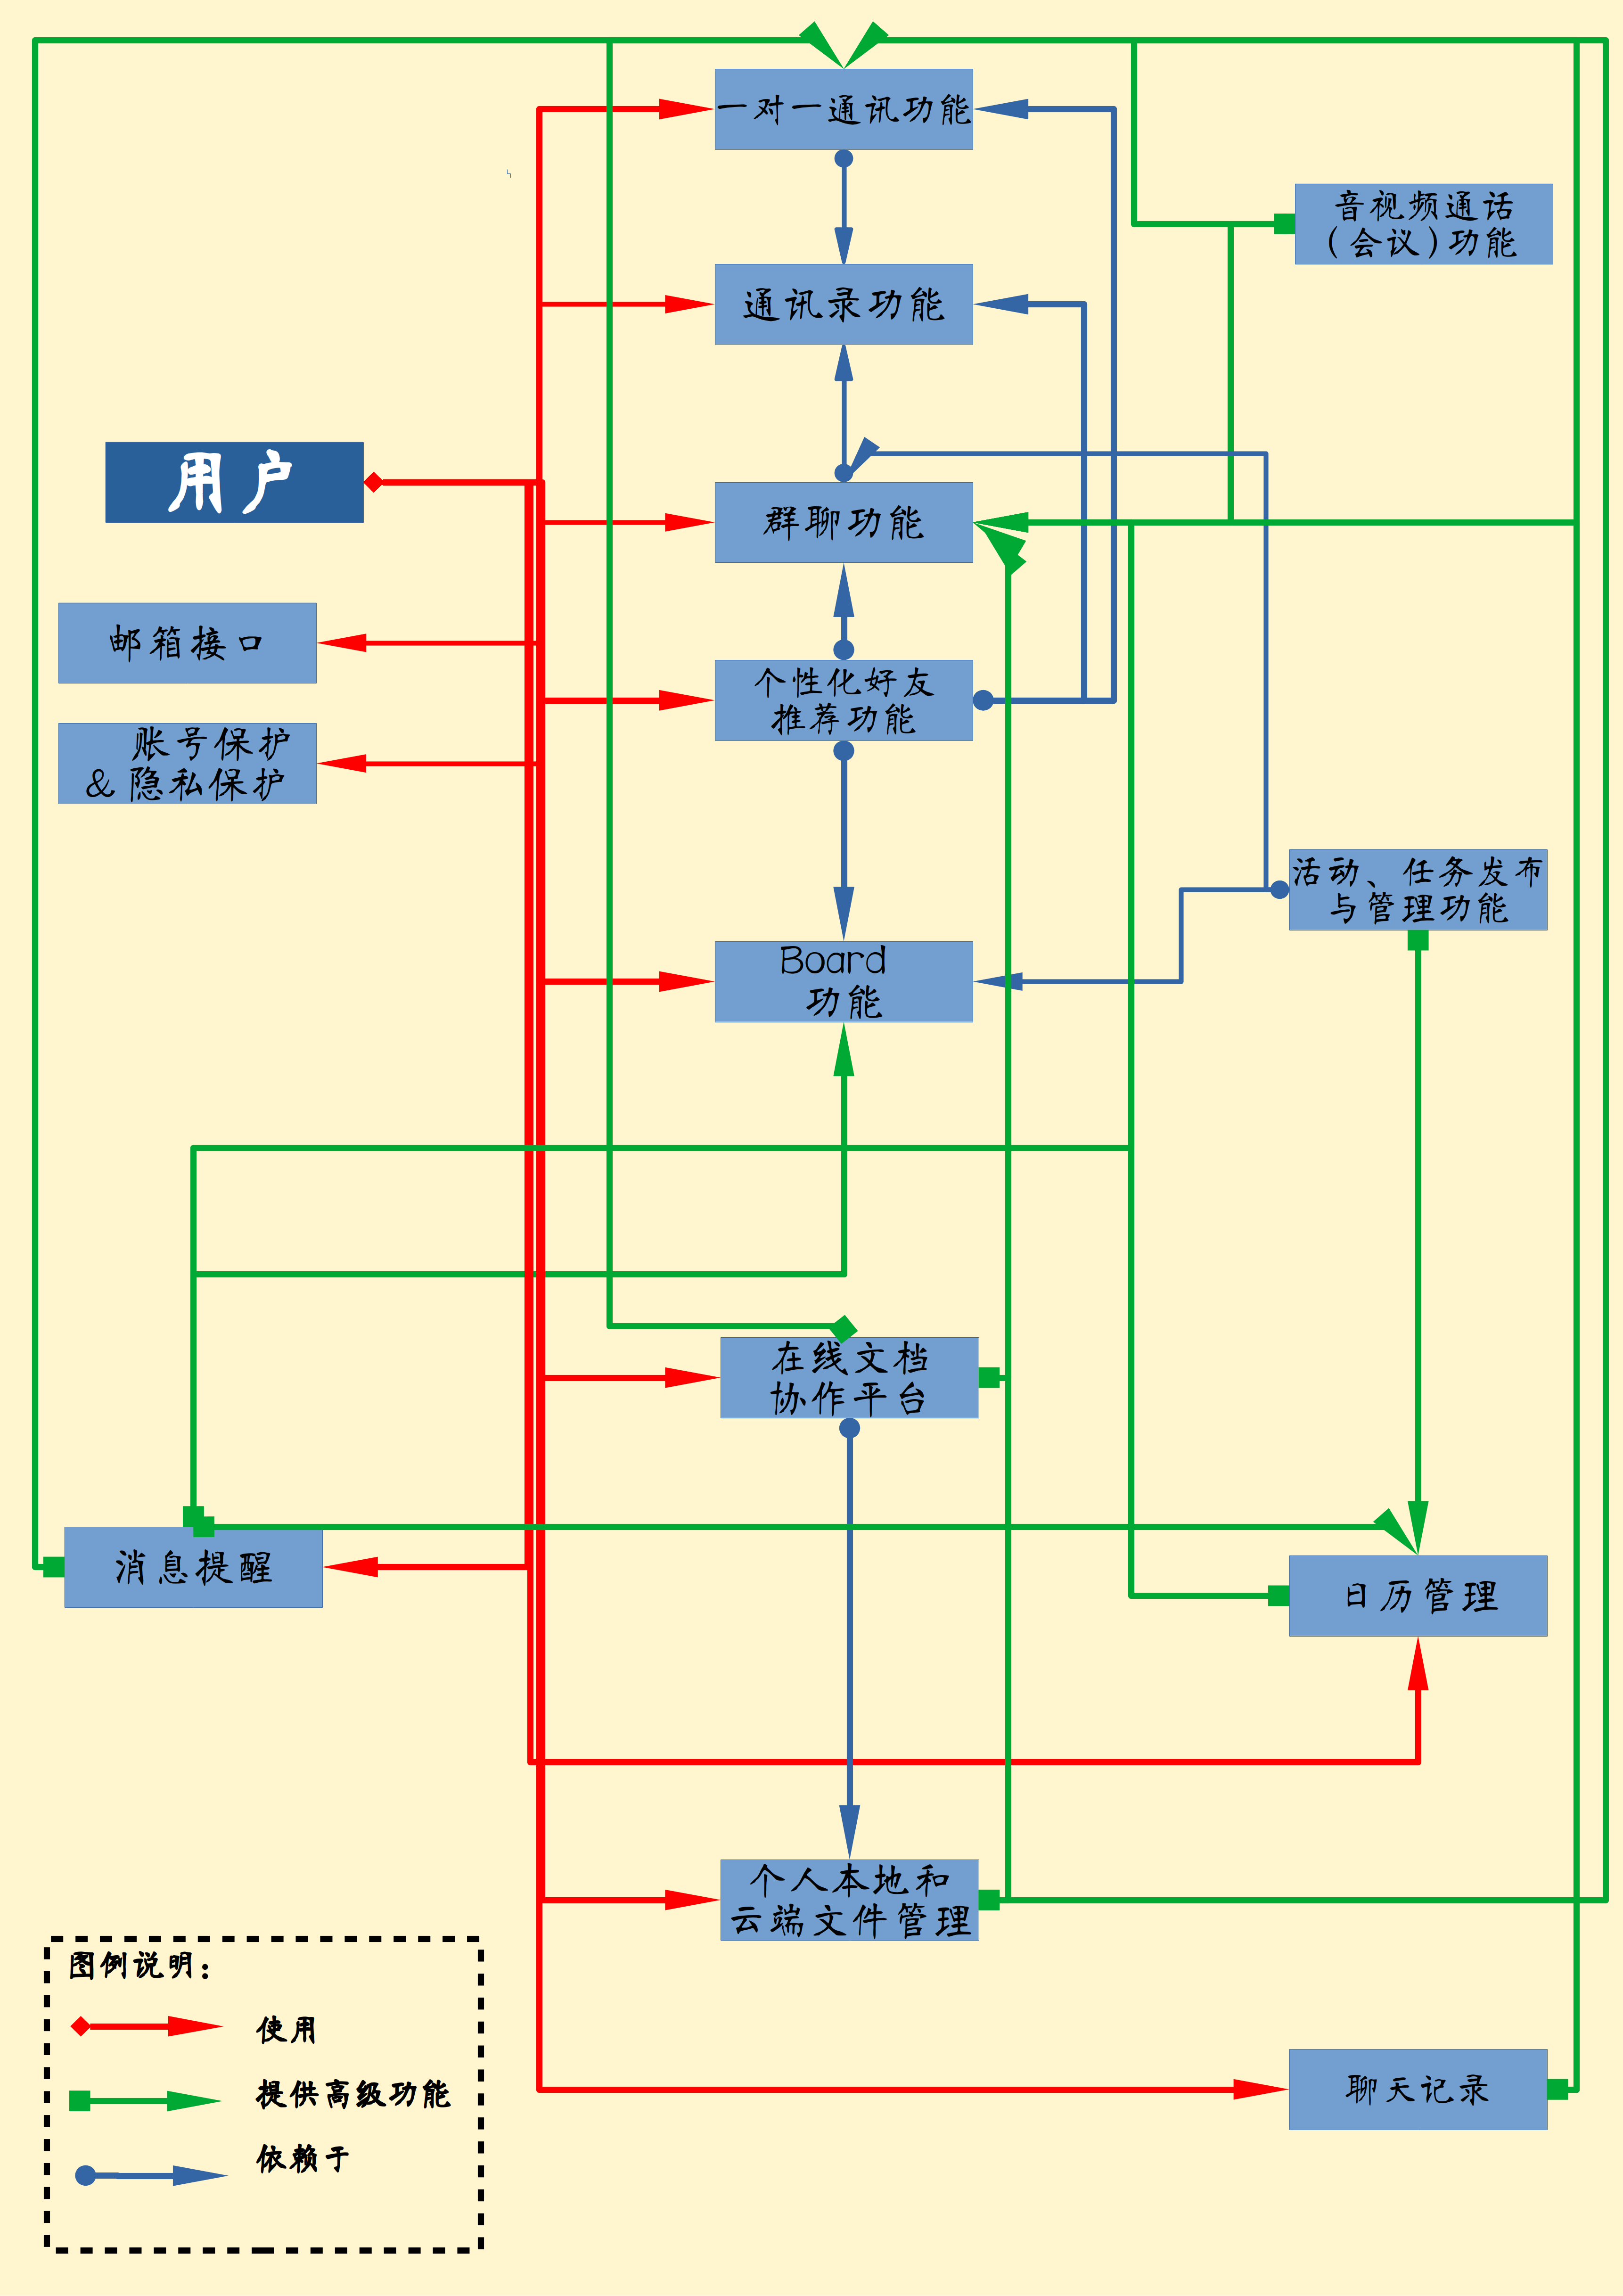
\includegraphics[scale = 0.75]{chat.png}
\end{center}
\section{用户特征}
%======================================================================================
% 列出对用户或系统操作者的要求,如:经验,能力,角色等。
% 本节不应描述具体需求。但本节内容是具体需求章节的基础。
%======================================================================================
\noindent
	本软件的主要目标人群包括:
	\begin{itemize}
		\item 高校大学生
		\item 科研机构研究人员
		\item 企业部门人员
		\item 工程开发团队人员
	\end{itemize}
	它主要适用于具有如下特点的人员:
	\begin{itemize}
		\item 在短期稳定的组织,如班级,实验室,团队
		\item 组织需要合作或者布置任务
		\item 需要合作编辑文档
		\item 需要频繁的信息沟通
		\item 定期开会
		\item 通信环境中有很多文件需要交换,发布、处理
		\item 有一些任务需要按时完成
		\item 日程安排严谨
		\item 对于所在环境(校园,公司)有社交需求
		\item 需要一定的通讯信息安全保证
		\item 有频繁、重要的邮件需要处理
	\end{itemize}
	针对以上用户特点,本软件可以高效,专业、全面地提供即时通讯及配套的各种功能。
\section{假设和依赖关系}
%======================================================================================
% 列出可能影响SRS中需求的所有的假设因素(与已知事实相对而言),
% 包括准备使用的第三方或商业组件,操作和开发环境的问题约束等。
% 如果上述假设不正确、没有被告知或者改变了都将对项目产生影响。
% 列出项目对外部条件的依赖,例如重用其他项目的模块等。
% 如果在其他文档(例如项目计划或范围文档等)里已经描述了,在这里可以不用描述。
%======================================================================================
\begin{itemize}                                                      
	\item 操作平台:Android,IOS,Windows,Linux
	\item 内部依赖关系:\\
		一对一通讯系统功能依赖于通讯录功能\\
		群聊功能依赖于通讯录功能\\
		个性化好友推荐功能依赖于一对一通讯功能、群聊功能、通讯录功能和Board功能\\
		在线文档协作平台依赖于个人文件和云端文件管理功能\\
		活动、任务发布与管理功能依赖于群聊功能和Board功能
	\item 外部依赖关系:\\
		邮箱接口功能依赖于外部邮箱组件
	\item 服务器端:借助第三方服务器
\end{itemize}
\chapter{具体需求}
\section{功能需求}
%====================================================================================================================
% 本子章节应描述软件产品的输入怎样被转换成输出。它描述了软件必须执行的基本动作。
% 对每一类功能或有时对每一个单独的功能,必须描述输入、处理、输出方面的需求。这些通常以下面四个子段落来组织:
% \subsubsection{介绍}
% 逐条列出与本特性相关的功能需求。包括项目如何响应预期的错误输入,非法条件和无效输入。需求应该简明,完整,不含糊,可验证,必要的。
% 当需要的信息不确定的时候使用“待定”。
% \subsubsection{输入}
% 本子段落应包含下列内容:
% A. 对该功能所有输入数据的详细描述,包括:
%	输入来源、数量、度量单位、时间要求、包含精度和容忍度的有效输入范围	
% B. 在适当的地方提供的对接口规格或接口控制文档的参考。
% \subsubsection{处理}
% 本子段落应描述对输入数据所执行的所有操作和如何获得输出的过程。这包括下列规格:
% A. 输入数据的有效性检测。
% B. 操作的确切次序,包括各事件的时序。
% C. 对异常情况的回应,例如:溢出、通信失败、错误处理
% D. 用于把系统输入转换到相应输出的任何方法(诸如方程式,数学算法,逻辑操作)。例如,这可能描述下列方面:
%	对工资单里代扣所得税的计算公式、用于气象预报的气象模型。	
% E. 对输出数据的有效性检测。
% \subsubsection{输出}
% 本子段落应包含:
% A. 对该功能所有输出数据的详细描述,这个描述包括:
%		输出的到何处(如打印机,文件)、数量、度量单位、时序、包含精确度和容忍度的有效输出范围
%		对非法值的处理、错误消息	
% B. 在适当的地方提供对接口规格或接口控制文档的参考。
% 此外,对那些需求集中在输入/输出行为的系统,SRS应描述所有重要的输入/输出行为及输入输出对的次序。
% 对一个需要记忆其行为以根据输入和过去的行为进行反应的系统,输入输出对的次序是要求的;这种功能行为就类似于有限状态机。
%====================================================================================================================
% 王浩宇
\subsection{一对一即时通讯}
\subsubsection{介绍}
\subsubsection{输入}
\subsubsection{处理}
\subsubsection{输出}
% 王浩宇
\subsection{R.INTF.CALC.002: 多情境群聊功能}
多种群聊场景支持:课程、班级、工程团队、工作小组
\subsubsection{介绍}
\subsubsection{输入}
\subsubsection{处理}
\subsubsection{输出}
% 戴路
\subsection{R.INTF.CALC.003: 活动/任务发布与管理功能}
\subsubsection{介绍}
\subsubsection{输入}
\subsubsection{处理}
\subsubsection{输出}
% 王浩宇
\subsection{R.INTF.CALC.004: 音视频通话(会议)功能}
\subsubsection{介绍}
\subsubsection{输入}
\subsubsection{处理}
\subsubsection{输出}
\subsection{R.INTF.CALC.005: 通讯录功能}
在日常使用中,我们一般不会和陌生人通信,而是和好友进行联系,或是在加入的群聊中发言。于是,我们使用通讯录管理所有的好友和群聊。
\subsubsection{介绍}
对用户而言,该功能的需求为:
\begin{itemize}
  \item 用户可以添加其他人为好友,可以通过账号查询、二维码等多种方式添加好友,向其发送好友请求。
  \item 用户可以加入群聊,可以通过账号查询、二维码等多种方式加入群聊,向其发送入群申请。
  \item 用户可以接受或拒绝其他用户的好友请求和入群邀请。
  \item 用户可以在通讯录中查询好友或群聊,进行通讯。
  \item 用户可以单方面删除好友。
  \item 用户可以退出群聊。
  \item 用户可以为好友进行分组。
  \item 用户可以将其他人加入或移出黑名单,用户不会接收来自黑名单的任何信息。
  \item 用户可以为好友增加备注信息。
\end{itemize}
\subsubsection{输入}
用户对好友的添加、删除和查询,用户设置的备注信息。
\subsubsection{处理}
\begin{itemize}
  \item \textbf{添加好友(群聊):} 可以根据提供的信息定位到具体的用户(群聊),向他发送请求。在他接受后,把他的信息加入通讯录。
  \item \textbf{删除好友:} 从用户的通讯录中删除该好友,同时从他的通讯录中删除用户信息。
  \item \textbf{退出群聊:} 从用户的通讯录中删除该群聊,同时从它的群成员中删除用户信息。
  \item \textbf{查询好友(群聊):} 从通讯录中找到对应的好友(群聊),可以采用遍历、二分查找、哈希等方法。
  \item \textbf{备注好友:} 为好友增加备注。
  \item \textbf{好友分组:} 在通讯录中对好友分组管理。
  \item \textbf{黑名单:} 屏蔽来自黑名单的所有信息。
\end{itemize}
\subsubsection{输出}
展示用户在上述操作后的新通讯录。

\subsection{R.INTF.CALC.006: 聊天记录功能}
在很多时候,用户需要之前的聊天内容。于是,我们提供了聊天记录功能。
\subsubsection{介绍}
对用户而言,该功能的需求为:
\begin{itemize}
  \item 允许用户查询聊天记录,且保持设备间同步。
  \item 允许用户导出聊天记录(txt格式、xls格式等)。
\end{itemize}
\subsubsection{输入}
对聊天记录的查询条件(时间、聊天对象、关键词等),以及导出命令和格式。
\subsubsection{处理}
\begin{itemize}
  \item 在用户聊天的同时,记录所有的聊天内容,存放在聊天记录中(聊天记录存储在云端)。
  \item 对用户提供的查询条件,检索聊天记录,返回对应的内容。
  \item 在导出时,将聊天记录以对应的格式写入文件。
\end{itemize}
\subsubsection{输出}
\begin{itemize}
  \item 向用户展示查询得到的聊天内容。
  \item 导出操作会输出一个写有聊天记录的文件。如果文件写入失败(目录不存在、存储已满等),向用户报错。
\end{itemize}

% 王浩宇
\subsection{消息提醒功能(R.INTF.CALC.007)}
\subsubsection{介绍}
\subsubsection{输入}
\subsubsection{处理}
\subsubsection{输出}
% 戴路
\subsection{Board(广场)功能(R.INTF.CALC.008)}
\subsubsection{介绍}
\subsubsection{输入}
\subsubsection{处理}
\subsubsection{输出}
\subsection{R.INTF.CALC.009: 个性化好友推荐功能}
为了扩大社交圈,用户需要更多的好友。于是,我们设计了该功能,为用户推荐志趣相投的好友。
\subsubsection{介绍}
对用户而言,该功能的需求为:
\begin{itemize}
  \item 用户可以输入一定的条件,系统会根据这些条件个性化地推荐好友
  \item 用户可以向推荐的好友发送好友请求
\end{itemize}
\subsubsection{输入}
好友选择条件。
\subsubsection{处理}
\begin{itemize}
  \item 根据用户平时的聊天信息、好友信息等,利用推荐算法得到一个用户集合。
  \item 根据用户的好友选择条件,从该集合中选择符合要求的用户子集。
  \item 从该子集中随机向用户输出五个符合要求的用户作为推荐的好友。
\end{itemize}
\subsubsection{输出}
向用户展示系统推荐的好友。
% 戴路
\subsection{在线文档协作平台}
\subsubsection{介绍}
\subsubsection{输入}
\subsubsection{处理}
\subsubsection{输出}
% 戴路
\subsection{账号保护 & 隐私保护}
\subsubsection{介绍}
\subsubsection{输入}
\subsubsection{处理}
\subsubsection{输出}
% 王浩宇
\subsection{R.INTF.CALC.012: 日历管理功能}
\subsubsection{介绍}
\subsubsection{输入}
\subsubsection{处理}
\subsubsection{输出}
% 王浩宇
\subsection{个人本地和云端文件管理}
\subsubsection{介绍}
\subsubsection{输入}
\subsubsection{处理}
\subsubsection{输出}
\subsection{R.INTF.CALC.014: 邮箱接口功能}
邮箱在日常生活中被广泛应用。于是,我们提供了邮箱接口功能。
\subsubsection{介绍}
对用户而言,该功能的需求为:
\begin{itemize}
  \item 用户可以为自己的账户绑定一个邮箱。
  \item 一旦邮箱收到新的邮件,就会给用户以消息提醒。
  \item 用户点击邮件按钮后,可以撰写邮件,并通过绑定的邮箱发送。
\end{itemize}
\subsubsection{输入}
用户绑定的邮箱,以及邮件信息。
\subsubsection{处理}
\begin{itemize}
  \item 在账户信息中增加一个条目,存储绑定的电子邮箱。
  \item 查询绑定的电子邮箱是否有邮件,一旦有邮件就调用消息提醒接口进行提醒。
  \item 读取用户输入的邮件信息,使用绑定的邮箱发送。
\end{itemize}
\subsubsection{输出}
使用消息提醒接口进行消息提醒。

\section{性能需求}
%====================================================================================================================
% 如果有性能方面的需求,在这里列出并解释他们的原理。以帮助开发者理解意图以做出正确的设计选择。在实时系统中的时序关系。保证需求尽可能的详细而精确。
%====================================================================================================================
\subsection{总体性能需求}

\subsubsection{支持的终端数目}
\begin{itemize}
	\item 移动端:1个;PC端:1 - 50个。
\end{itemize}
\subsubsection{支持的同时使用的用户数目}
\begin{itemize}
	\item 服务器集群可以支持不少于1000万用户同时在线使用。
\end{itemize}
\subsubsection{处理的文件和记录的数目}
\begin{itemize}
	\item 单个用户云端存储:文本$\geq$ 10000个,图片$\geq$ 1000000张,音视频$\geq$ 1000段,历史记录$\geq$ 500000条
	\item 单个用户单次处理(发送,上传):文本$\leq$ 50个,图片$\leq$ 20张,音视频$\leq$ 10段,历史记录$\leq$ 50条
	\item 群文件:文本$\geq$ 100000个,图片$\geq$ 10000000张,音视频$\geq$ 10000段,历史记录$\geq$ 5000000条
	\item 群文件单次处理(发送,上传):文本$\leq$ 500个,图片$\leq$ 200张,音视频$\leq$ 100段,历史记录$\leq$ 500条
\end{itemize}
\subsubsection{表和文件的大小}
\begin{itemize}
	\item 单个文件$\leq$ 10GB
\end{itemize}
\subsubsection{同时处理的事务数量}
同时处理的事务(功能请求,消息发送,文件上传)数量:
\begin{itemize}
	\item 客户端:$\leq$ 15个
	\item 服务器端:$\geq$ $10^{8}$ 个
\end{itemize}
\subsubsection{正常信息发送延迟}
正常信息(客户端处理器不繁忙,网络传输速度$\geq$ 10KB/s)发送延迟 $\leq$ 0.30s。
\subsubsection{正常操作响应时间}
正常操作(客户端处理器不繁忙,网络传输速度$\geq$ 10KB/s)响应时间 $\leq$ 0.15s。
\subsubsection{平台适应性}
本系统提供安卓移动客户端,IOS移动客户端,WindowsPC客户端,Linux操作系统客户端版本。
\subsubsection{内存占用限制}
正常工作状态(平均状态)内存占用$\leq$ 256MB, 峰值状态内存占用$\leq$ 512MB,平稳无操作状态下自动结束无用进程。
% \subsubsection{正常工作状态耗电限制}

\subsection{具体功能的性能需求}
某些具体功能不仅需要满足上述的总体性能需求,还需要满足下面的额外性能需求。如果某功能没有在下面提到,那么它没有任何额外的性能需求。

\textbf{音视频通话:} 为了保证通话的流畅性,总时延应当$\leq$0.1s。总时延指的是某一帧视频从被录制到在对方处播放所经过的时间。

\textbf{通讯录:} 对单个用户而言,通讯录应当支持不少于10000位好友(黑名单)。

\textbf{账号保护和隐私保护功能:} 在发送邮件进行验证时,邮件应当在10s内到达绑定的邮箱。

% \subsubsection{一对一即时通讯}
% \subsubsection{群聊}
% \subsubsection{活动/任务发布与管理}
%====================================================================================================================
% 本子章节应从整体上描述静态和动态的量化的对软件(或人与软件交互)的需求。
% 静态的量化需求可能包括:
%	A. 支持的终端数目。
%	B. 支持的同时使用的用户数目。
%	C. 处理的文件和记录的数目。
%	D. 表和文件的大小。
% 动态的量化需求可能包括:
%	A. 在正常和峰值工作量条件下特定时间段(如一小时)
%	B. 处理的事务和任务的数目以及数据量。
% 所有的这些需求应以可测量的术语进行描述,例如所有的操作应在1秒内被处理完成,而不是描述成操作员不必等待操作的完成。
% 注意: 用于一个具体功能的量化限制通常在该功能的处理子章节中描述。
%====================================================================================================================
\section{外部接口需求}
\subsection{用户接口}
%====================================================================================================================
% 详细描述系统与用户之间的接口
% 这应描述下述内容:
% A. 对每种人机界面,软件所必须支持的特性。例如,如果系统用户通过一个显示终端进行操作,那么应包含下述内容:
% 	要求的屏幕格式、页面规划及报告或菜单的内容
%	输入和输出的相关时序、一些组合功能键的用法
% B. 与系统用户接口使用相关的所有方面。这可能只是一个简单的关于系统怎样展示给用户而该做什么和不该做什么的列表。
%	例如提供关于长或短错误消息选项。和所有其它需求一样,这些需求也应能被检验,
%	例如,四级打字员经一小时的培训后能在Z分钟内完成功能X,而不是一个打字员能完成功能X。
%====================================================================================================================

\subsection{软件接口}
\subsubsection{移动端}
	\begin{enumerate}
		\item 操作系统平台:Android 4.0以上,IOS 6以上
		\item 开发语言:JAVA
		\item 开发工具:Eclipse IDE 2019‑03
	\end{enumerate}
\subsubsection{PC端}
	\begin{enumerate}
		\item 操作系统平台:Windows7以上,Linux4.1.0以上,IOS 6以上
		\item 开发语言:JAVA
		\item 开发工具:Eclipse IDE 2019‑03
	\end{enumerate}
\subsubsection{服务器端}
	借助第三方服务器
%====================================================================================================================
% 详细描述与其他系统 /模块 /项目之间的接口
% 在此应描述如何使用其它(必需的)软件产品(例如,数据管理系统,操作系统,或算法工具包),
% 以及与其它应用系统的接口(例如,协议处理系统和数据库管理系统之间的接口)。
% 对每个必需的软件产品,应提供下列信息:
%	A. 名字、B. 助记符、C. 版本号、 D. 来源
% 对每个接口,本部分应:
%	A .	讨论与本软件产品相关的接口软件的目的。
%	B.	按消息/函数内容和格式定义接口。如果接口已在其它文档中很清楚地描述,就没有必要在这儿进行详细描述,但需说明应参考的文档。
%====================================================================================================================
\subsection{硬件接口}
\subsubsection{移动端}
	\begin{enumerate}
		\item 处理器要求:MSM800系列,Exynos5433以上,HelioX10以上,麒麟系列,A8以上
		% \item 运行环境:Android 4.0以上,IOS 6以上
		\item 内存要求:512MB以上
	\end{enumerate}
\subsubsection{PC端}
	\begin{enumerate}
		\item 处理器要求:Intel® Core™ i5以上
		% \item 运行环境:jdk11.0
		\item 内存要求:512MB以上
	\end{enumerate}
%====================================================================================================================
% 详细描述与硬件的接口
% 在此描述软件产品和系统硬件组件之间接口的逻辑特征,也包括支持哪些设备、怎样支持这些设备和协议等。
% 按软/硬件协议内容和格式定义接口。如果接口已在其它文档中很清楚地描述,就没有必要在这儿进行详细描述,但需说明应参考的文档。
%====================================================================================================================
\subsection{通讯接口}
使用TCP协议进行通讯,参考RFC793(https://tools.ietf.org/html/rfc793)。
%====================================================================================================================
% 详细描述通讯接口,如本地网络协议等。
% 按消息/函数内容和格式定义接口。如果接口已在其它文档中很清楚地描述,就没有必要在这儿进行详细描述,但需说明应参考的文档。
%====================================================================================================================

\chapter{总体设计约束}
<Describe any items or issues that will limit the options available to the developers. >

描述可能限制开发人员选择的事项。
 
\section{标准符合性}
< This subsection should specify the requirements derived from existing standards or regulations. In case, if the project refers any International standards, then the deviations from the standards could be specified along with the International standards reference. >

本节详细说明需求所采用的标准或规范的来源。如果项目采用了国际标准,应该说明国际标准及项目与标准的偏离情况。

\section{硬件约束}
<This subsection could include Requirements for the software to operate inside various hardware constraints, such as timing constraints, memory constraints etc.)

本节包括软件在不同的硬件平台运行的需求,如时间相关的约束,内存方面的约束等。

\section{技术限制}
<This subsection could include limitations on the use of specific technologies, interfaces, databases, parallel operations; communications protocols; design conventions or programming standards. >

本节包括对使用特定技术的限制,包括接口,数据库,并行操作,通讯协议,设计约定,编程规范等。

\chapter{软件质量特性}
%======================================================================================
% 详细说明项目任何其他的质量特性。该特性对客户和开发者都非常重要。
% 考虑的方面包括:适应性,可用性,正确性,灵活性,交互工作能力,可维护性,可移植性,可靠性,
% 可重用性,鲁棒性,可测试性和可用性等。定量的详细描述这些特性,尽可能的可验证。
% 对不同属性之间的重要性加以阐述,如:易用性比易学性更重要。
% 每一个属性单独使用一个小节描述,可根据需要进行增减,如增加可维护性小节等。
%======================================================================================
\begin{enumerate}
    \item 正确性:
    \item 可靠性:
    \item 效率:
    \item 完整性:
    \item 易使用性:
    \item 可维护性:
    \item 可测试性:
    \item 复用性:
    \item 安全保密性:
    \item 可理解性:
    \item 互联性:要求网络条件正常,不低于10KB/s
\end{enumerate}


\chapter{其他需求}
%======================================================================================
% 使用适当的章节,详细说明任何其他客户需求,包括数据库,编码需求,错误处理,测试需求等。
%======================================================================================
\section{编码需求与代码可维护性}
%======================================================================================
    统一Unicode编码;符合JAVA程序开发规范,清晰简明易维护,注释量不少于总代码量40\%;安装程序
    自动检测平台依赖,一键安装方便快捷,一键卸载不留残余。
%======================================================================================
\section{错误处理}
%======================================================================================
\noindent
    客户端: \\
        1. 产生的任何错误不能损害用户数据或损害平台上的其他数据\\
        2. 在设备掉电、系统崩溃的情况下保护好用户数据\\
        3. 及时向服务器发送错误信息\\
    服务器端:\\
        1. 使用安全稳定可靠的第三方服务器\\
        2. 及时处理客户端发送的错误信息维护代码
%======================================================================================
\section{增量更新能力}
%======================================================================================
    客户端软件升级/更新支持增量更新,避免频繁下载安装包重装。
%======================================================================================
\section{数据库}
%======================================================================================
% 详细说明项目相关的数据库方面的需求。
%======================================================================================
    采用Oracle18.3数据库系统,合理设计数据库系统,要求能进行数据库的建立,调优,重组,重构,
    安全管控,报错问题的分析、汇总和处理、日常备份。
\section{操作}
%======================================================================================
% 详细说明用户通常的和特殊的操作需求。
%======================================================================================
\noindent
用户基本操作方式:\\
    1. 标准鼠标键盘\\
    2. 触屏\\
    3. 语音控制\\
用户核心操作支持:\\
    1. 文字信息处理发送\\
    2. 图片文件编辑发送\\
    3. 音视频录制发送\\
用户其他常用操作支持:  \\
    1. 浏览Board信息\\
    2. 添加删除好友,加群退群\\
    3. 查看隐私内容或安全属性\\
    4. 管理日历\\
    5. 通过邮箱接口管理邮件\\
用户特殊操作支持:\\
    1. 自动更新\\
    2. 卸载\\
    3. 报告错误\\
    4. 修改隐私内容或安全属性
\section{本地化}
%======================================================================================
% 描述支持多语种的需求。
%======================================================================================
支持中文(简体)、中文(繁体)、英文、法文,俄文,阿拉伯文。
\chapter{\color{red}依赖关系}
%======================================================================================
% 解释每一条需求的内部和外部依赖关系。
%======================================================================================
\begin{table}[htbp]
    \centering
    %======================================================================================
    \caption{\color{red}依赖关系表} \label{tab:classification}
    %======================================================================================
    \begin{tabular}{|p{6em}|p{9em}|p{9em}|p{7em}|}
            \hline%---------------------------------------------------------------------------------------------------------------
            依赖关系ID  & 功能                                     & 被依赖的功能                              & 依赖说明 \\
            \hline%---------------------------------------------------------------------------------------------------------------
            001        & 个性化好友推荐(R.INTF.CALC.009)           & 一对一通讯功能(R.INTF.CALC.001)            & 推荐有频繁联系的非好友联系人\\
            \hline%---------------------------------------------------------------------------------------------------------------
            002        & 个性化好友推荐(R.INTF.CALC.009)           & 群聊功能(R.INTF.CALC.002)                 & 推荐相同群聊中的非好友联系人\\
            \hline%---------------------------------------------------------------------------------------------------------------
            003        & 个性化好友推荐(R.INTF.CALC.009)           & 通讯录功能(R.INTF.CALC.005)               & 推荐相同群聊中的非好友联系人\\
            \hline%---------------------------------------------------------------------------------------------------------------
            004        & 个性化好友推荐(R.INTF.CALC.009)           & Borad功能(R.INTF.CALC.008)               & 推荐频繁互相访问的非好友联系人\\
            \hline%---------------------------------------------------------------------------------------------------------------
            005        & 一对一通讯功能(R.INTF.CALC.001)           & 通讯录功能(R.INTF.CALC.005)               & 确定通讯对象\\
            \hline%---------------------------------------------------------------------------------------------------------------
            006        & 群聊功能(R.INTF.CALC.002)                & 通讯录功能(R.INTF.CALC.005)               & 确定通讯对象\\
            \hline%---------------------------------------------------------------------------------------------------------------
            007        & 在线文档协作平台(R.INTF.CALC.010)         & 个人本地和云端文件管理功能(R.INTF.CALC.013)  & 提供云端文件管理服务\\
            \hline%---------------------------------------------------------------------------------------------------------------
            008        & 活动/任务发布与管理功能(R.INTF.CALC.003)   & Borad功能(R.INTF.CALC.008)               & 获取活动/任务信息\\
            \hline%---------------------------------------------------------------------------------------------------------------
            009        & 活动/任务发布与管理功能(R.INTF.CALC.003)   & 群聊功能(R.INTF.CALC.002)                 & 获取活动/任务信息\\
            \hline%---------------------------------------------------------------------------------------------------------------
            010        & 邮箱接口功能(R.INTF.CALC.014)            & 第三方邮件插件                             & 管理邮件\\
            \hline%---------------------------------------------------------------------------------------------------------------
                \color{red}011        
            &   \color{red}流程审批功能(R.INTF.CALC.015)            
            &   \color{red}通讯录功能(R.INTF.CALC.005)                
            &   \color{red}获取审批人信息       \\
            \hline%---------------------------------------------------------------------------------------------------------------
    \end{tabular}
\end{table}
\begin{table}[htbp]
    \centering
    %======================================================================================
    \caption{\color{red}依赖关系表(续)} \label{tab:classification}
    %======================================================================================
    \begin{tabular}{|p{6em}|p{9em}|p{9em}|p{7em}|}
            \hline%---------------------------------------------------------------------------------------------------------------
            依赖关系ID  & 功能                                     & 被依赖的功能                              & 依赖说明 \\
            \hline%---------------------------------------------------------------------------------------------------------------
                \color{red}012        
            &   \color{red}流程审批功能(R.INTF.CALC.015)            
            &   \color{red}消息提醒功能(R.INTF.CALC.007)                
            &   \color{red}向审批人提醒审批申请,返回提醒申请人申请结果\\
            \hline%---------------------------------------------------------------------------------------------------------------
                \color{red}013        
            &   \color{red}流程审批功能(R.INTF.CALC.015)            
            &   \color{red}账号保护和隐私保护功能(R.INTF.CALC.011)                
            &   \color{red}保护审批信息\\
            \hline%---------------------------------------------------------------------------------------------------------------
                \color{red}014        
            &   \color{red}信息调研功能(R.INTF.CALC.016)            
            &   \color{red}Borad功能(R.INTF.CALC.008)                           
            &   \color{red}确定调查人群\\
            \hline%---------------------------------------------------------------------------------------------------------------
                \color{red}015        
            &   \color{red}信息调研功能(R.INTF.CALC.016)            
            &   \color{red}群聊功能(R.INTF.CALC.002)                           
            &   \color{red}确定调查人群\\
            \hline%---------------------------------------------------------------------------------------------------------------
                \color{red}016        
            &   \color{red}信息调研功能(R.INTF.CALC.016)            
            &   \color{red}通讯录功能(R.INTF.CALC.005)                            
            &   \color{red}确定调查人群\\
            \hline%---------------------------------------------------------------------------------------------------------------
                \color{red}017 
            &   \color{red}第三方账号同步功能(R.INTF.CALC.017)            
            &   \color{red}消息提醒功能(R.INTF.CALC.007)                             
            &   \color{red}第三方新消息提醒\\
            \hline%---------------------------------------------------------------------------------------------------------------
                \color{red}018        
            &   \color{red}第三方账号同步功能(R.INTF.CALC.017)            
            &   \color{red}账号保护和隐私保护功能(R.INTF.CALC.011)                             
            &   \color{red}保护用户第三方账号信息安全\\
            \hline%---------------------------------------------------------------------------------------------------------------
    \end{tabular}
\end{table}
\chapter{需求分级}
\begin{table}[htbp]
\centering
\caption{需求分级表} \label{tab:classification}
\begin{tabular}{|c|c|c|}
    \hline
    需求ID & 需求名称 & 需求分级 \\
    \hline
    a & b & c \\
    \hline
    a & b & c \\
    \hline
    a & b & c \\
    \hline
    a & b & c \\
    \hline
    a & b & c \\
    \hline
    a & b & c \\
    \hline
    a & b & c \\
    \hline
    a & b & c \\
    \hline
\end{tabular}
\end{table}

Importance of requirements are classified as following:
\begin{enumerate}
\item Mandatory: absolutely essential features, without which the product development will be canceled.
\item Important: unessential features that may affect the viability of the product.
\item Nice to have: desired features, the absence of which will not affect the product viability.
\end{enumerate}

重要性分类如下:
\begin{itemize}
\item 必须的		绝对基本的特性;如果不包含,产品就会被取消。
\item 重要的		不是基本的特性,但这些特性会影响产品的生存能力。
\item 最好有的		期望的特性;但省略一个或多个这样的特性不会影响产品的生存能力
\end{itemize}

\chapter{待确定问题}
%======================================================================================
    \begin{table}[htbp]
        \centering
        %======================================================================================
            \caption{待确定问题表} \label{tab:tbd_problems}
        %======================================================================================
        \begin{tabular}{|p{8em}|p{5em}|p{3em}|p{5em}|p{3em}|p{2em}|p{5em}|}
                \hline
                需求ID & 问题描述 & 影响(H/M/L) & 风险 & 责任人 & 解决日期 & 状态(Open/Close) \\
                \hline
                R.INTF.CALC.001 & 使用第三方服务器 & H & 服务器宕机 & 王浩宇 & -- & Open\\
                \hline
                R.INTF.CALC.004 & 信息流不稳定 & M & 信息流不稳定 & 王浩宇 & -- & Open\\
                \hline
                R.INTF.CALC.010 & 编辑一致性 & M & 冲突编辑 & 张劲暾 & -- & Open\\
                \hline
                R.INTF.CALC.013 & 安全性 & M & 非法入侵与资料盗取 & 戴路 & -- & Open\\
                \hline
                    \color{red}R.INTF.CALC.017 
                &   \color{red}第三方网站无法访问 
                &   \color{red}L 
                &   \color{red}该功能无法提供 
                &   \color{red}戴路 
                &   \color{red}-- 
                &   \color{red}Open  \\
                \hline
            \end{tabular}
    \end{table}
%======================================================================================

%\chapter{Latex使用例子}

\section{图}
\subsection{示例}
\begin{figure}[ht]
\centering

\includegraphics[width=10cm]{ustc_logo_fig}
\caption{测试图片} \label{fig:figure1}
\end{figure}

\subsection{带图注的图}
\begin{figure}[ht]
\centering

\includegraphics[width=10cm]{ustc_logo_fig}
\caption{带图注的图片}\label{fig:noted-figure}
\note{the solid lines represent the time histogram of the spontaneous activities of an old monkey cell(gray) and a young monkey cell (black). The bin-width is 1}
\end{figure}

\section{表格}

\subsection{A Simple Table}
\begin{table}[htbp]
\centering
\caption{这里是表的标题} \label{tab:simpletable}
\begin{tabular}{|c|c|}
    \hline
    a & b \\
    \hline
    c & d \\
    \hline
\end{tabular}
\note{这里是表的注释}
\end{table}

\subsection{长表格}
\begin{longtable}{ccc}
% 首页表头
\caption[长表格演示]{长表格演示} \label{tab:longtable} \\
\toprule[1.5pt]
名称  & 说明 & 备注\\
\midrule[1pt]
\endfirsthead
% 续页表头
\caption[]{长表格演示(续)} \\
\toprule[1.5pt]
名称  & 说明 & 备注 \\
\midrule[1pt]
\endhead
% 首页表尾
\hline
\multicolumn{3}{r}{\small 续下页}
\endfoot
% 续页表尾
\bottomrule[1.5pt]
\endlastfoot

AAAAAAAAAAAA   &   BBBBBBBBBBB   &   CCCCCCCCCCCCCC   \\
AAAAAAAAAAAA   &   BBBBBBBBBBB   &   CCCCCCCCCCCCCC   \\
AAAAAAAAAAAA   &   BBBBBBBBBBB   &   CCCCCCCCCCCCCC   \\
AAAAAAAAAAAA   &   BBBBBBBBBBB   &   CCCCCCCCCCCCCC   \\
AAAAAAAAAAAA   &   BBBBBBBBBBB   &   CCCCCCCCCCCCCC   \\
AAAAAAAAAAAA   &   BBBBBBBBBBB   &   CCCCCCCCCCCCCC   \\
AAAAAAAAAAAA   &   BBBBBBBBBBB   &   CCCCCCCCCCCCCC   \\
AAAAAAAAAAAA   &   BBBBBBBBBBB   &   CCCCCCCCCCCCCC   \\
AAAAAAAAAAAA   &   BBBBBBBBBBB   &   CCCCCCCCCCCCCC   \\
AAAAAAAAAAAA   &   BBBBBBBBBBB   &   CCCCCCCCCCCCCC   \\
AAAAAAAAAAAA   &   BBBBBBBBBBB   &   CCCCCCCCCCCCCC   \\
AAAAAAAAAAAA   &   BBBBBBBBBBB   &   CCCCCCCCCCCCCC   \\
AAAAAAAAAAAA   &   BBBBBBBBBBB   &   CCCCCCCCCCCCCC   \\
AAAAAAAAAAAA   &   BBBBBBBBBBB   &   CCCCCCCCCCCCCC   \\
AAAAAAAAAAAA   &   BBBBBBBBBBB   &   CCCCCCCCCCCCCC   \\
AAAAAAAAAAAA   &   BBBBBBBBBBB   &   CCCCCCCCCCCCCC   \\
AAAAAAAAAAAA   &   BBBBBBBBBBB   &   CCCCCCCCCCCCCC   \\
AAAAAAAAAAAA   &   BBBBBBBBBBB   &   CCCCCCCCCCCCCC   \\
AAAAAAAAAAAA   &   BBBBBBBBBBB   &   CCCCCCCCCCCCCC   \\
AAAAAAAAAAAA   &   BBBBBBBBBBB   &   CCCCCCCCCCCCCC   \\
AAAAAAAAAAAA   &   BBBBBBBBBBB   &   CCCCCCCCCCCCCC   \\
AAAAAAAAAAAA   &   BBBBBBBBBBB   &   CCCCCCCCCCCCCC   \\
AAAAAAAAAAAA   &   BBBBBBBBBBB   &   CCCCCCCCCCCCCC   \\
AAAAAAAAAAAA   &   BBBBBBBBBBB   &   CCCCCCCCCCCCCC   \\
AAAAAAAAAAAA   &   BBBBBBBBBBB   &   CCCCCCCCCCCCCC   \\
AAAAAAAAAAAA   &   BBBBBBBBBBB   &   CCCCCCCCCCCCCC   \\
AAAAAAAAAAAA   &   BBBBBBBBBBB   &   CCCCCCCCCCCCCC   \\
AAAAAAAAAAAA   &   BBBBBBBBBBB   &   CCCCCCCCCCCCCC   \\
AAAAAAAAAAAA   &   BBBBBBBBBBB   &   CCCCCCCCCCCCCC   \\
AAAAAAAAAAAA   &   BBBBBBBBBBB   &   CCCCCCCCCCCCCC   \\
AAAAAAAAAAAA   &   BBBBBBBBBBB   &   CCCCCCCCCCCCCC   \\
AAAAAAAAAAAA   &   BBBBBBBBBBB   &   CCCCCCCCCCCCCC   \\
AAAAAAAAAAAA   &   BBBBBBBBBBB   &   CCCCCCCCCCCCCC   \\
AAAAAAAAAAAA   &   BBBBBBBBBBB   &   CCCCCCCCCCCCCC   \\
AAAAAAAAAAAA   &   BBBBBBBBBBB   &   CCCCCCCCCCCCCC   \\
AAAAAAAAAAAA   &   BBBBBBBBBBB   &   CCCCCCCCCCCCCC   \\
\end{longtable}


\section{算法环境}
模板中使用 \texttt{algorithm2e} 宏包实现算法环境。关于该宏包的具体用法,
请阅读宏包的官方文档。

\begin{algorithm}[htbp]
\SetAlgoLined
\KwData{this text}
\KwResult{how to write algorithm with \LaTeX2e }

initialization\;
\While{not at end of this document}{
    read current\;
    \eIf{understand}{
        go to next section\;
        current section becomes this one\;
    }{
        go back to the beginning of current section\;
    }
}
\caption{算法示例1}
\label{algo:algorithm1}
\end{algorithm}

\IncMargin{1em}
\begin{algorithm}
\SetKwData{Left}{left}\SetKwData{This}{this}\SetKwData{Up}{up}
\SetKwFunction{Union}{Union}\SetKwFunction{FindCompress}{FindCompress}
\SetKwInOut{Input}{input}\SetKwInOut{Output}{output}

\Input{A bitmap $Im$ of size $w\times l$}
\Output{A partition of the bitmap}
\BlankLine
\emph{special treatment of the first line}\;
\For{$i\leftarrow 2$ \KwTo $l$}{
    \emph{special treatment of the first element of line $i$}\;
    \For{$j\leftarrow 2$ \KwTo $w$}{\label{forins}
        \Left$\leftarrow$ \FindCompress{$Im[i,j-1]$}\;
        \Up$\leftarrow$ \FindCompress{$Im[i-1,]$}\;
        \This$\leftarrow$ \FindCompress{$Im[i,j]$}\;
        \If(\tcp*[h]{O(\Left,\This)==1}){\Left compatible with \This}{\label{lt}
            \lIf{\Left $<$ \This}{\Union{\Left,\This}}
            \lElse{\Union{\This,\Left}}
        }
        \If(\tcp*[f]{O(\Up,\This)==1}){\Up compatible with \This}{\label{ut}
        \lIf{\Up $<$ \This}{\Union{\Up,\This}}
        \tcp{\This is put under \Up to keep tree as flat as possible}\label{cmt}
        \lElse{\Union{\This,\Up}}\tcp*[h]{\This linked to \Up}\label{lelse}
        }
    }
    \lForEach{element $e$ of the line $i$}{\FindCompress{p}}
}
\caption{算法示例2}\label{algo_disjdecomp}
\label{alog:algorithm2}
\end{algorithm}\DecMargin{1em}


\section{代码环境}
模板中使用 \texttt{listings} 宏包实现代码环境。详细用法见宏包的官方说明文档。

以下是代码示例,可以在文中任意位置引用\autoref{first-code} 。
\begin{lstlisting}[language=C, caption=示例代码, label={code:first-code}]
#include <stdio.h>

int main( )
{
    printf("hello, world\n");
    return 0;
}
\end{lstlisting}




\section{引用文献标注}

\subsection{著者-出版年制标注法}

\noindent
\verb|\citestyle{ustcauthoryear}|
\citestyle{ustcauthoryear}

\noindent
\begin{tabular}{l@{\quad$\Rightarrow$\quad}l}
  \verb|\cite{knuth86a}| & \cite{knuth86a}\\
  \verb|\citet{knuth86a}| & \citet{knuth86a}\\
  \verb|\citet[chap.~2]{knuth86a}| & \citet[chap.~2]{knuth86a}\\[0.5ex]
  \verb|\citep{knuth86a}| & \citep{knuth86a}\\
  \verb|\citep[chap.~2]{knuth86a}| & \citep[chap.~2]{knuth86a}\\
  \verb|\citep[see][]{knuth86a}| & \citep[see][]{knuth86a}\\
  \verb|\citep[see][chap.~2]{knuth86a}| & \citep[see][chap.~2]{knuth86a}\\[0.5ex]
  \verb|\citet*{knuth86a}| & \citet*{knuth86a}\\
  \verb|\citep*{knuth86a}| & \citep*{knuth86a}\\
\end{tabular}

\noindent
\begin{tabular}{l@{\quad$\Rightarrow$\quad}l}
  \verb|\citet{knuth86a,tlc2}| & \citet{knuth86a,tlc2}\\
  \verb|\citep{knuth86a,tlc2}| & \citep{knuth86a,tlc2}\\
  \verb|\cite{knuth86a,knuth84}| & \cite{knuth86a,knuth84}\\
  \verb|\citet{knuth86a,knuth84}| & \citet{knuth86a,knuth84}\\
  \verb|\citep{knuth86a,knuth84}| & \citep{knuth86a,knuth84}\\
\end{tabular}

\subsection{顺序编码制标注法}

\noindent
\verb|\citestyle{ustcnumerical}|
\citestyle{ustcnumerical}

\noindent
\begin{tabular}{l@{\quad$\Rightarrow$\quad}l}
  \verb|\cite{knuth86a}| & \cite{knuth86a}\\
  \verb|\citet{knuth86a}| & \citet{knuth86a}\\
  \verb|\citet[chap.~2]{knuth86a}| & \citet[chap.~2]{knuth86a}\\[0.5ex]
  \verb|\citep{knuth86a}| & \citep{knuth86a}\\
  \verb|\citep[chap.~2]{knuth86a}| & \citep[chap.~2]{knuth86a}\\
  \verb|\citep[see][]{knuth86a}| & \citep[see][]{knuth86a}\\
  \verb|\citep[see][chap.~2]{knuth86a}| & \citep[see][chap.~2]{knuth86a}\\[0.5ex]
  \verb|\citet*{knuth86a}| & \citet*{knuth86a}\\
  \verb|\citep*{knuth86a}| & \citep*{knuth86a}\\
\end{tabular}

\noindent
\begin{tabular}{l@{\quad$\Rightarrow$\quad}l}
  \verb|\citet{knuth86a,tlc2}| & \citet{knuth86a,tlc2}\\
  \verb|\citep{knuth86a,tlc2}| & \citep{knuth86a,tlc2}\\
  \verb|\cite{knuth86a,knuth84}| & \cite{knuth86a,knuth84}\\
  \verb|\citet{knuth86a,knuth84}| & \citet{knuth86a,knuth84}\\
  \verb|\citep{knuth86a,knuth84}| & \citep{knuth86a,knuth84}\\
  \verb|\cite{knuth86a,knuth84,tlc2}| & \cite{knuth86a,knuth84,tlc2}\\
\end{tabular}

\subsection{其他形式的标注}

\noindent
\begin{tabular}{l@{\quad$\Rightarrow$\quad}l}
  \verb|\citealt{tlc2}| & \citealt{tlc2}\\
  \verb|\citealt*{tlc2}| & \citealt*{tlc2}\\
  \verb|\citealp{tlc2}| & \citealp{tlc2}\\
  \verb|\citealp*{tlc2}| & \citealp*{tlc2}\\
  \verb|\citealp{tlc2,knuth86a}| & \citealp{tlc2,knuth86a}\\
  \verb|\citealp[pg.~32]{tlc2}| & \citealp[pg.~32]{tlc2}\\
  \verb|\citenum{tlc2}| & \citenum{tlc2}\\
  \verb|\citetext{priv.\ comm.}| & \citetext{priv.\ comm.}\\
\end{tabular}

\noindent
\begin{tabular}{l@{\quad$\Rightarrow$\quad}l}
  \verb|\citeauthor{tlc2}| & \citeauthor{tlc2}\\
  \verb|\citeauthor*{tlc2}| & \citeauthor*{tlc2}\\
  \verb|\citeyear{tlc2}| & \citeyear{tlc2}\\
  \verb|\citeyearpar{tlc2}| & \citeyearpar{tlc2}\\
\end{tabular}

\nocite{*}
\bibliography{bib/tex}

\appendix
\chapter{可行性分析结果}
%======================================================================================
% 描述对分配需求的可行性分析结果。
%======================================================================================
\section{技术可行性}
%======================================================================================
    技术可行性分析主要分析现有技术条件能否顺利完成开发工作,软硬件配置能否满足
    开发者需求。即时通讯系统的主要功能是提供现代工作场景下信息交互,通知发布,团队组织、
    任务管理的平台解决方案。所依赖的的安卓、IOS、Windows、Linux操作系统,Intel和智能移动端硬件平台,JAVA开发语言和
    Eclipse开发环境都是成熟的开发生态圈,技术上可行。
%======================================================================================
\section{经济可行性}
%======================================================================================
    经济可行性上,本团队人力成本相对大型互联网企业偏低,场地使用学校实验室不需
    要支付额外的费用,开发除了硬件消耗,服务器租用,软件维护的少量费用以外,
    不存在其余开发费用。启动资金在个人承受范围以内,经营成本相对低。通过广告、
    融资之后硬件和人力经济压力也会有所缓解,因此经济上具有可行性。
%======================================================================================
\section{法律可行性}
%======================================================================================
\begin{itemize}
    \item 侵犯专利权:无
    \item 侵犯版权:无
\end{itemize}
%======================================================================================
\section{可行性分析结论}
%======================================================================================
    随着现代社会发展与互联网产业崛起,高等院校、科研机构、企业部门和开发团队对于即时通讯平台的功能和
    性能需求与日俱增,需要一个保证即时通讯效率,提供不同团队模式合作、场景应用、信息发布,任务管理,文档管理
    与在线合作功能的解决方案。根据以上分析可知,开发面向工作团队的即时通讯系统有着稳定可靠的技术、经济和
    法律可行性,将带来巨大的社会价值和良好的商业应用前景。所以,我们认为开发这个平台的条件已经具备,可以开始开发工作。
%======================================================================================
\chapter{需求建模 }
\section{数据流图}
\subsection{顶层数据流图}
<Draw the Top-level DFD here>

在这里画出顶层数据流图

\subsection{层数据流图}
<Draw the Level-0 DFD here>

在这里画出0层数据流图

\subsection{层数据流图}
<Draw the Level-1 DFD here>

在这里画出1层数据流图

\section{数据字典}
\subsection{数据流说明}
\subsubsection{数据流1名称}
<Title of  the data flow should accord with the one in data flow diagram, and the Data description notions should be used.  >

与数据流图中的名称一致,采用数据描述符号说明数据流的内容

\subsubsection{数据流2名称}
<Title of  the data flow should accord with the one in data flow diagram, and the Data description notions should be used   >

与数据流图中的名称一致,采用数据描述符号说明数据流的内容

\subsection{数据存储说明}
\subsubsection{数据存储1名称}
<Title of  the data flow should accord with the one in data flow diagram, and the Data description notions should be used. The arrangement of the data in data store should also be described.>

与数据流图中的名称一致,采用数据描述符号说明数据流的内容,另外还需描述数据排列方式

\subsubsection{数据存储2名称}
<Title of  the data flow should accord with the one in data flow diagram, and the Data description notions should be used.The arrangement of the data in data store should also be described.>

与数据流图中的名称一致,采用数据描述符号说明数据流的内容,另外还需描述数据排列方式

\subsection{加工说明}
\subsubsection{加工1名称}
<Use natural language, Decision table/Decision tree and Pseudocode to describe how to process the data flow>

采用自然语言,判断表/判断树,伪码的形式描述对数据流进行处理的过程

\subsubsection{加工2名称}
<Use natural language, Decision table/Decision tree and Pseudocode to describe how to process the data flow>

采用自然语言,判断表/判断树,伪码的形式描述对数据流进行处理的过程



\end{document}
